\documentclass[10pt,a4paper,twocolumn,twoside]{article}
\usepackage[utf8]{inputenc}
\usepackage[catalan]{babel}
\usepackage{multicol}
\usepackage{graphicx}
\usepackage{fancyhdr}
\usepackage{times}
\usepackage{titlesec}
\usepackage{multirow}
\usepackage{lettrine}
\usepackage[top=2cm, bottom=1.5cm, left=2cm, right=2cm]{geometry}
\usepackage[figurename=Fig.,tablename=TAULA]{caption}
\captionsetup[table]{textfont=sc}

\author{\LARGE\sffamily Daniel Ortega Berja}
\title{\Huge{\sffamily RUNTIME INTRUSION DETECTION SYSTEM}}
\date{}

\newcommand\blfootnote[1]{%
  \begingroup
  \renewcommand\thefootnote{}\footnote{#1}%
  \addtocounter{footnote}{-1}%
  \endgroup
}

%
%\large\bfseries\sffamily
\titleformat{\section}
{\large\sffamily\scshape\bfseries}
{\textbf{\thesection}}{1em}{}

\begin{document}

\fancyhead[LO]{\scriptsize DANIEL ORTEGA BERJA: RUNTIME INTRUSION DETECTION SYSTEM}
\fancyhead[RO]{\thepage}
\fancyhead[LE]{\thepage}
\fancyhead[RE]{\scriptsize EE/UAB TFG INFORMÀTICA: RUNTIME INTRUSION DETECTION SYSTEM}

\fancyfoot[CO,CE]{}

\fancypagestyle{primerapagina}
{
   \fancyhf{}
   \fancyhead[L]{\scriptsize TFG EN ENGINYERIA INFORMÀTICA, ESCOLA D'ENGINYERIA (EE), UNIVERSITAT AUTÒNOMA DE BARCELONA (UAB)}
   \fancyfoot[C]{\scriptsize Febrer de 2021, Escola d'Enginyeria (UAB)}
}

%\lhead{\thepage}
%\chead{}
%\rhead{\tiny EE/UAB TFG INFORMÀTICA: RUNTIME INTRUSION DETECTION SYSTEM)}
%\lhead{ EE/UAB \thepage}
%\lfoot{}
%\cfoot{\tiny{February 2015, Escola d'Enginyeria (UAB)}}
%\rfoot{}
\renewcommand{\headrulewidth}{0pt}
\renewcommand{\footrulewidth}{0pt}
\pagestyle{fancy}

%\thispagestyle{myheadings}
\twocolumn[\begin{@twocolumnfalse}

%\vspace*{-1cm}{\scriptsize TFG EN ENGINYERIA INFORMÀTICA, ESCOLA D'ENGINYERIA (EE), UNIVERSITAT AUTÒNOMA DE BARCELONA (UAB)}

\maketitle

\thispagestyle{primerapagina}
%\twocolumn[\begin{@twocolumnfalse}
%\maketitle
%\begin{abstract}
\begin{center}
\parbox{0.915\textwidth}
{\sffamily
\textbf{Resum--}
Monitoritzar el kernel de Linux en temps d'execucio per detectar modificacions no desitjades, per aixo s'tilitzara una tecnologia de virtualització per poder crear una capa per sota del SO de manera que el codi que s´hi trobi estigui aïllat i protegit. Tenint en compte que el codi ha de tenir un bon rendiment, haura d'adaptar-se a la carrega del sistema si s'escau i fer menys comprovacions en moments que l'us dels recursos del sistema es elevat.
\\
\\
\textbf{Paraules clau-- } Kernel, modificacions, ciberseguretat, arquitectura de computadors.\\
\\

%\end{abstract}
%\bigskip
%\begin{abstract}
\bigskip
\\
\textbf{Abstract--} Monitor the Linux kernel at runtime to detect undesirable modifications, so a virtualization technology will be used to create a layer below the OS so that the code in it is isolated and protected. Given that the code must perform well, it will have to adapt to the system load if necessary and do fewer checks at times when the use of system resources is high.
\\
\\
\textbf{Keywords-- }Kernel, Modifications, CyberSecurity, Computer Architecture.\\

}

\bigskip

{\vrule depth 0pt height 0.5pt width 4cm\hspace{7.5pt}%
\raisebox{-3.5pt}{\fontfamily{pzd}\fontencoding{U}\fontseries{m}\fontshape{n}\fontsize{11}{12}\selectfont\char70}%
\hspace{7.5pt}\vrule depth 0pt height 0.5pt width 4cm\relax}

\end{center}


\bigskip
%\end{abstract}
\end{@twocolumnfalse}]

\blfootnote{$\bullet$ E-mail de contacte: danielortegaberja@gmail.com}
\blfootnote{$\bullet$ Menció realitzada: Tecnologies de la Informació}
\blfootnote{$\bullet$ Treball tutoritzat per: Angel Elbaz (DEIC)}
\blfootnote{$\bullet$ Curs 2020/2021}
\section{Introducció}
\lettrine[lines=3]{P}otser parlar tambe de prevenció i detecció.(situar com era abans un atac amb exemple i un com es ara, potser explicar meltdown i spectre)
A mesura que els anys passen, la tecnologia és més avançada i, per tant, complex. Els sistemes de seguretat també han anat millorant, posant més difícil als ciberdelinqüents atacar un sistema. És per això que tant les tècniques d’atac com de defensa de sistemes es fan més sofisticats i es busquen noves maneres per protegir un sistema de possibles atacs. De fet, es poden trobar casos en els quals es fa ús de cadenes d’eines no conegudes públicament per atacar empreses, aquestes cadenes inclouen noves vulnerabilitats que els experts en seguretat han de saber detectar a temps per estalviar danys inesperats.[1]
\subsection{Què són els hipervisors i la virtualització}
El concepte de virtualització es basa en crear una capa de software que permeti a programes o fins i tot a sistemes operatius executar-se concurrentment, de manera que queden aïllats entre ells però dins d’una mateixa màquina.
Aquesta nova capa actua d’interfície entre les altres, emulant o adaptant el comportament que tindrien les crides de capes superiors a inferiors (instruccions màquina, crides al sistema, llibreries...), és a dir, tenim diferents conceptes de virtualització segons la capa on s’apliquen. [3]

\subsection{Què és el nucli d'un Sistema Operatiu}
El nucli d’un sistema operatiu és el conjunt d’aplicacions encarregat de gestionar la memòria, gestionar els processos, controlar els dispositius i fer les crides al sistema, una capa transparent entre el hardware i els processos.
Així doncs, el codi de detecció de modificacions s’executarà en el VMM amb un espai de memòria diferent del del sistema operatiu podent comprovar amb periodicitat les possibles modificacions del nucli del sistema operatiu a examinar, en aquest cas Linux.
\subsection{Què és un sistema d'intrusions}
Els sistemes de detecció d’intrusions es focalitzen en l’anàlisi de comportaments anòmals del sistema i en el posterior avís a un administrador. D’aquesta manera, mitjançant la monitorització de diferents variables es poden descobrir possibles accessos no controlats a un sistema, detectant així quan un intrús faci modificacions del sistema.
Segons les mètriques triades un sistema de detecció serà:
\begin{itemize}
\item Network-Based: Monitoritza tot el tràfic anòmal de xarxa d’entrada i sortida.
\item Host-Based: Analitza diferents esdeveniments dins d’un mateix hoste.
\end{itemize}
En aquest projecte es farà un servir un sistema de detecció de tipus Host-Based, per tant, s’haurà d’elaborar un programa que monitoritzi el sistema hoste. És molt important l’entorn on s’executarà aquest programa, ja que si volem que sigui fiable i inalterable haurà d’estar separat dels mateixos tipus d’atacs al que estigui sotmès el sistema a protegir.

Els tipus de detecció d’intrusions generals solen ser basats en signatures, en estadístiques de comportament (ús de Machine Learning), o estats preguardats del sistema per comparar-los amb els estats actuals [2]. Actualment, no està decidit quin serà el tipus de detecció i s’està investigant en noves formes no compresses en aquests punts.

\section{Objectius}
L'objectiu del projecte serà monitoritzar el kernel de Linux en temps d'execució per detectar modificacions no desitjades, per això s'utilitzarà una tecnologia de virtualització per poder crear una capa per sota del SO de manera que el codi que s´hi trobi estigui aïllat i protegit. Tenint en compte que el codi ha de tenir un bon rendiment, haurà d'adaptar-se a la càrrega del sistema si s'escau i fer menys comprovacions en moments que l'ús dels recursos del sistema és elevat. Separant per punts els objecitus del projecte:
\begin{itemize}
\item Entendre l’arquitectura de tecnologies de virtualització i hipervisors.
\item Entendre el funcionament de cada mòdul del kernel de Linux.
\item Modificar i extendre un monitor de màquines virtuals Open-Source
\item Implementar un codi de detecció i monitorització.
\item Aconseguir que el codi detecti en temps d’execució.
\item Observar l’impacte en rendiment que tingui el nostre codi a l’equip instal·lat.
\item Adaptar el codi a uns nivells de rendiments acceptables segons el sistema.
\end{itemize}

També es contempla opcionalment poder implementar més d'un sistema de deteccioó, poder adaptar el codi al requisits hardware d'una impresora i observar el nou impacte en rendiment que hi trobariem per posteriorment adaptar la càrrega que afegeixi el sistema.
\section{Estat de l'art}

\section{Metodologia}

Durant l'execució d'aquest projecte s'han adaptat diferents fases segons les necessitats tècniques de cada part de la implementació, és a dir, en moments del projecte on la dificultat era major, el balanç entre fases ha pogut variar pero en general sempre han seguit la mteixa estructura.

En primer lloc la cerca d'informació ha estat organitzada de duess maneres, cada cop que una tasca era planificada es reservava un interval de temps suficientment ample perquè aquesta tasca deixès madurar els conceptes que es buscaven, a mès, un cop trobats s'havien de redactar en esborrany abans de la següent etapa. En segon lloc es posava en pràctica els conceptes apressos per avançar en l'objectiu principal del projecte, permetent modificacions i nous plantejaments però sempre deixant versions estables que vagin avançant per no perdre el fil del projecte. Finalment, podem dir que a nivell de projecte i per fer reunions es feia servir una metodologia basa en SCRUM personalitzada, fent l'estructura esmentada anteriorment en una setmana de duració, així les funcionalitats anaven integran-se en el projecte i era sempre funcional.

Altres metodologies utilitzades com per poder seguir un bon ritme de treball, han estat fer servir tècniques de gestió del temps com temporitzadors Pomodoro on els intervals de treballs eren de 50 minuts i els descans de 10. I finalment esmentar l'ús d'eines de control de versions per desenvolupament software com GitHub, això ha servit per poder tenir la seguretat de no patir imprevistos i perdre parts del projecte, també el fet de tenir una branca principal i una altra per fer proves ha agilitzat molt per veure la diferència entre versions, l'última avantatge que ens ha atorgat l'entorn Git es poder fer ullades al codi sense necessitat de muntar tot l'entorn de desenvolupament. 

\section{Resultats}



\section{Accès a les pàgines del kernel}
Qualsevol dels dispositius utilitzats avui en dia porta un sistema operatiu, des d’smartphones fins a ordinadors basen les seves aplicacions i el seu funcionament segons el S.O que utilitzin. Aquest sistema operatiu està composat per diferents components que el formen, però sera el nucli (en anglès Kernel) la part principal d’ell. Per l’usuari això serà una capa totalment transparent, on nomès podrà percebra la part gràfica de tot el conjunt de components que conformen la lògica d’un ordinador.

\begin{figure}[!h]
\centering
	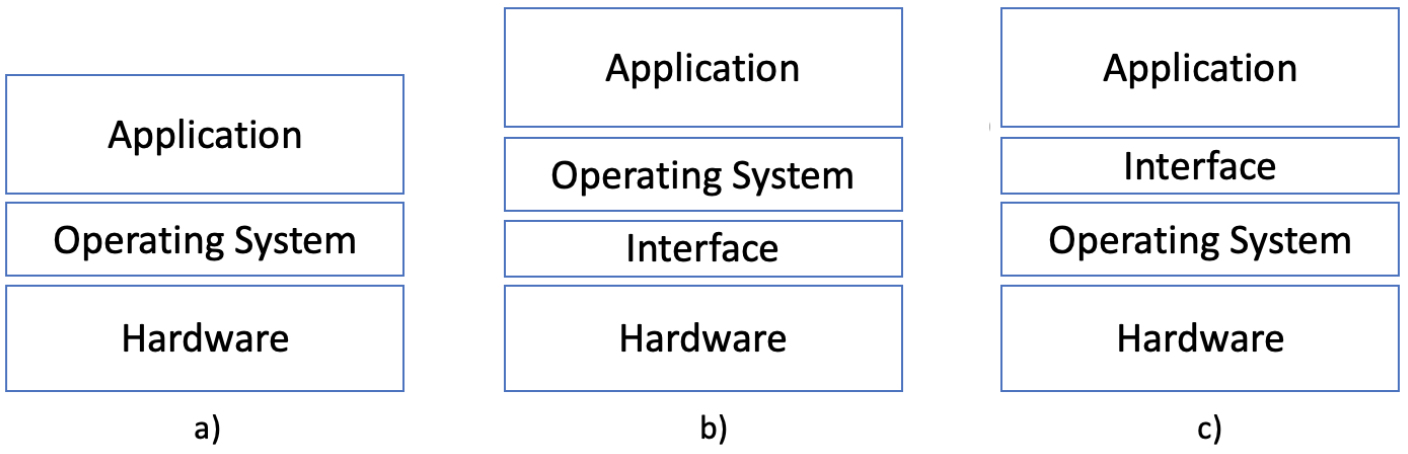
\includegraphics[width=0.45\textwidth]{06-InformeFinal-Latex/img/arquitectura.png}
	\caption{Exemple de figura}
	\label{fig-exemple}
\end{figure}

Com es pot veure a la figura 1-3 existeixen 3 capes que conformen l’ordinador: capa d’aplicació, el sistema operatiu i el hardware, i serà nomès la primera amb la que l’usuari es podrà comunicar. Desprès de la seqüència d’inici del sistema, el nucli Linux és el primer en ser iniciat i per atendre a totes les tasques del sistema es llencen processos concurrents, aquests demanen recursos ja sigui de connectivitat, de còmput, memòria, etc. Especifiquem doncs, que el nucli es el codi encarregat d’orquestrar el consum de recursos del hardware que demanen els processos de les aplicacions.
Ja sigui d’un sistema operatiu Windows, Mac o ara bé de qualsevol distribució basada en Linux el nucli funciona com a interfície entre els esmentats processos i el hardware del sistema encarregant-se de 5 grans tasques:

\begin{itemize}
\item Gestionar la memòria: El tamany de memòria de l’ordinador és immens i s’estableixen polítiques per poder accedir a diferents rangs de memòria de la manera que més rendiment s’obtingui. Per evitar haver de fer cerques innecessàries i disposar de més espai de memòria en els processos és fa ús de la memòria virtual i es gestionada pel gestor de memòria del nucli, més endevant s’explicarà amb més detall l’espai virtual de memòria. 
\item Gestionar els processos: S’estableixen mitjançant planificador de tasques, quins processos poden fer ús del recursos de la CPU i per quant temps, també estableix com es comuniquen els processos entre ells (senyals, pipes …).
\item Controladors de dispositius: Actua com a mediador amb cada perifèric connectat al sistema, estableix totes les operacions de control sobre els dispositius que s’esta utilitzant.
\item Xarxa: Entrada i sortida de paquets, esdeveniments asíncrons, i en general totes les operacions de la xarxa han de ser classificats i identificats abans que un procès els utilitzi. El sistema és l’encarregat del control de la resolució d’adreces i de distribuir la informació per les interfícies de xarxa.
\item Crides al sistema: Eines utilitzades per les aplicacions per comuinicar-se amb el sistema operatiu.

\end{itemize}
A mès també estableix el sistema de fitxers on defineix l’estàndard necessari segons les necessitats del sistema, comprèn una gran varietat de formats, per tant, portar un sistema de fitxer a Linux és molt més fàcil que a altres kernels.
En el plantejament inicial, es tenia clar que es volia fer un sistema d’intrusions de tipus Host-Based, és a dir, que s’analitzarien diferents esdeveniments dins del mateix hoste, per tant, no s’analitzaria la part del nucli corresponent a la xarxa i es miraria quin dels altres aspectes del nucli es poden monitoritzar: memòria, processos, controladors o crides al sistema.
Com podem imiaginar, el nucli del sistema conté el codi essencial i inalterable del sistema, qualsevol aplicació farà ús de les crides al sistema operatiu o funcions del nucli i, per tant, qualsevol alteració en aquell codi pot tenir un impacte crític en el funcionament del nostre sistema. S’enfoca, doncs, el sistema de detecció de moficiació en la comprovació de l’existencia de nomès codi legítim al nucli, per això s’investigarà en la gestió de memòria qe fa el nucli i dels permissos que ha de tenir.
\subsection{Sistema de paginació}
Quan s’executa un programa, no es fa ús de direccions físiques de memòria, sino de direccions lògiques establertes en els sistemes per especificar adreces d’operacions o intstruccions, aquestes tenen un format segmentat i segons la seva longitud i tipus poden interpretar-se de maneres diferents. En comú tenen que cada conjunt de l’adreça identifica un nivell de segment de dades i un desplaçament que es fa a partir del segment esmentat. La seva notació pot trobar-se en hexadecimal de 32 bits o 64 bits.
\begin{itemize}
\item Adreça Lineal de 32 bits: 0x00002000
\item Adreça Lineal de 64 bits: 0xFFFF800000000000
\end{itemize}

L’arquitectura del nostre sistema és Intel IA-32e, es duu a terme la traducció d’adreces lineals en estructures geràrquiqes de pàginació a travès del registre CR3. Tot i disopsar de 64 bits a les adreces, aquesta arquitectura nomès en fa ús de 48 a 52 bits de cada direcció, amb 48 bits adrecem 256TBytes d’espai d’adreces lineals i amb 52 es podria arribar a 4PBytes, per tant es veu com no es neccessari fer ús de tot l’espai comprès pels 64 bits.

\begin{figure}[!h]
\centering
	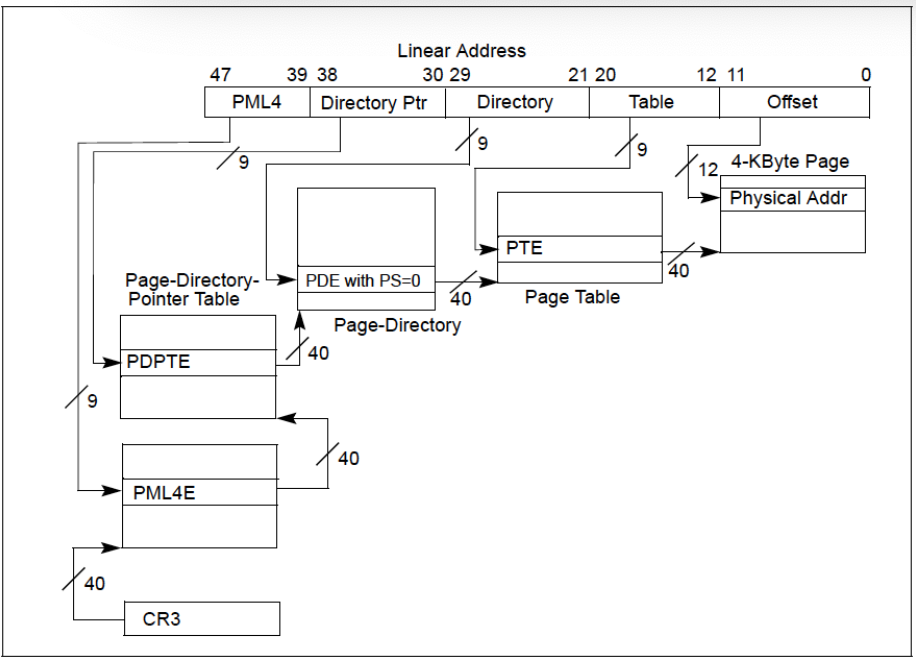
\includegraphics[width=0.45\textwidth]{06-InformeFinal-Latex/img/paginacio.png}
	\caption{Exemple de figura}
	\label{NivellsPaginacio}
\end{figure}


L’estructura geràrquica esmentada anteriorment i observada a la figura 1-4, es separa en 4 nivells: Page Map Level 4 (PML4), Page Directory Pointer Table (PDPT), Page Directory Table (PDT) i Page Table (PT) on es troben totes les entrades que apunten a les següents taules. Segons el tamany de la pàgina de destinació la distrbució de bits per cada nivell de paginació es diferent. Per trobar la pàgina d’una direcció lògica en concret es segueix el següent procès:

TAULA

\begin{itemize}
\item Obtenció PML4: Per poder accedir a la direcció lineal de la taula de nivell 4 s’agafen els bits 51:12 del registre CR3, seguidament es treu l’entrada concreta de la taula amb els btis 47:39 de l’adreça lineal a analitzar, finalment es sumen els dos ultims bits amb valor 0.
\item Obtenció PDPT: Seguidament agafgem els bits 51:12 de la direcció que es troba a l’entrada de la PML4 (PML4e), concatenem els bits 38:30 de la direcció lineal i dos zeros.
\item Obtenció PT: Per obtenir l’entrada del Page Directory agafem també els bits 51:12 de l’adreça física que es troba a l’entrada, els traduïm a lògica per poder sumar l’índex d’entrada corresponent als bits 29:21 de la direcció lineal i afegim dos bits a 0 al final.
\end{itemize}
POSSIBLE IMATGE

A la figura 1-5 es pot observar la distribució de bits per cada adreça segons el nivell, a més de l’espai corresponent als bits 51:12 on es troba l’adreça del següent nivell, també trobem entre el bit 1 i 8 alguns dels flags que analitzarem per trobar el codi desitjat. Tot i que parlarem més endevant de quins d’aquests analitzem els bits més comuns són present, lectura/escritura, pwt, pcd, accessed, dirty, pat i global.



\subsection{Mapes de memòria i registres}

\section{Emmagatzematge dels resultats}
\subsection{Anàlisi}
Un cop es pot accedir a les pàgines corresponents al nucli del sistema, farem una comprovació sobre els permissos que tenen pel seu contingut. Els atributs de les pàgines esmentats poden ser executable (X) o no-executable (NX) i Read-Write (R/W) o Read-Only (RO).
Volem comprovar que el codi pertinent al kernel no ha estat modificat i es farà una comprovació que miri que totes les pàgines amb permissos de supervisor, estigui marcat com a executable i sigui nomès de lectura (RO). També comprovarem que cap codi no legítim és inserit i per tant s’haurà de comprovar que cap pàgina amb permissos NX ara en té de X i també que les pàgines que abans tenien l’atribut executable són les mateixes que ara ho tenen.
Anterioment hem parlat de la distribuciío i significats dels bits en les direccions lògiques i els més comuns per posició son els següents:

% Utilitzeu el begin table només en cas de vole taules flotants. Si les voleu al lloc, tabular directament.
\begin{table}
\caption{Taula d'exemple}
\label{tab:senzilla}
\begin{center}
\resizebox{\columnwidth}{!}{%

\begin{tabular}{|c||c|c|c|c|c|c|c|c|}
\hline

\multicolumn{9}{ |c| }{Distribució bits a direccions lògiques} \\
\hline
Número bit & 1 & 2 & 3 & 4 & 5 & 6 & 7 & 8 \\
\hline
Contingut & Present & R/W & PWT & PCD & Acessed & Dirty & PAT & Global\\

\hline
\end{tabular}
}
\end{center}
\end{table}



TAULA
(tambexplicar aqui com es relaciona amb el KPTI)


El Page Table Isolation (de les sigles PTI en anglès) és una mesura de defensa aplicada a partir de la vulnerabilitat Meltdown descoberta al 2018 que afectaba a totes les CPU que existien fins al moment. Aquest atac aprofitaba una vulnerabilitat que permetia llegir codi del nucli independentment de la distribució dels espais d’adreces [11]. Per tant, aquesta mesura afecta al plantejament inicial del projecte, on es pretenia accedir a l’espai d’adreces del nucli disponible a la mateixa taula que el d’adreces, ara s’implementen dos taules on quan s’està en mode privilegiat es disposa de tot el conjunt d’espai d’adreces i en mode usuar nomès hi ha el contingut indispensable de codi del nucli pel funcionament del sistema. Val a dir que aquest espai disponible encara posa en risc el sistema, posant a disposició el valor d’alguns punters i, per tant, l’aleatorietat del sistema.

\begin{figure}[!h]
\centering
	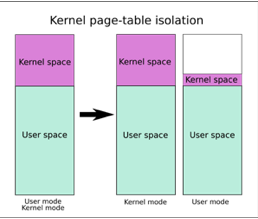
\includegraphics[width=0.45\textwidth]{06-InformeFinal-Latex/img/KPTI.png}
	\caption{Exemple de figura}
	\label{KPTI}
\end{figure}

Per plantejar la nova formar de poder accedir a aquestes pàgines es va investigar en una part concreta de l’hipervisor, en concret la part de codi que es comunica amb el gestor de memòria del nucli. En ella trobem documentat que per aquest hipervisor existeix un mapa de memòria (que guarda com està distribuida la memòria del sistema) i que conté totes les direccions de taules de pàgina del kernel per la màquina virtual. De fet, segons indiquen els mètodes de la classe, pot retornar mapejat el registre CR3 en aquest mapa de memòria per poder accedir a totes les entrades. Quedant-nos la següent distribució:

Per tant, en comptes de fer l’accès anterior on obteníem el mapa de memòria i el CR3 d’allà, primer intentarem que al CR3 estigui mapejat el que apunta a les direccions del kernel.

\begin{figure}[!h]
\centering
	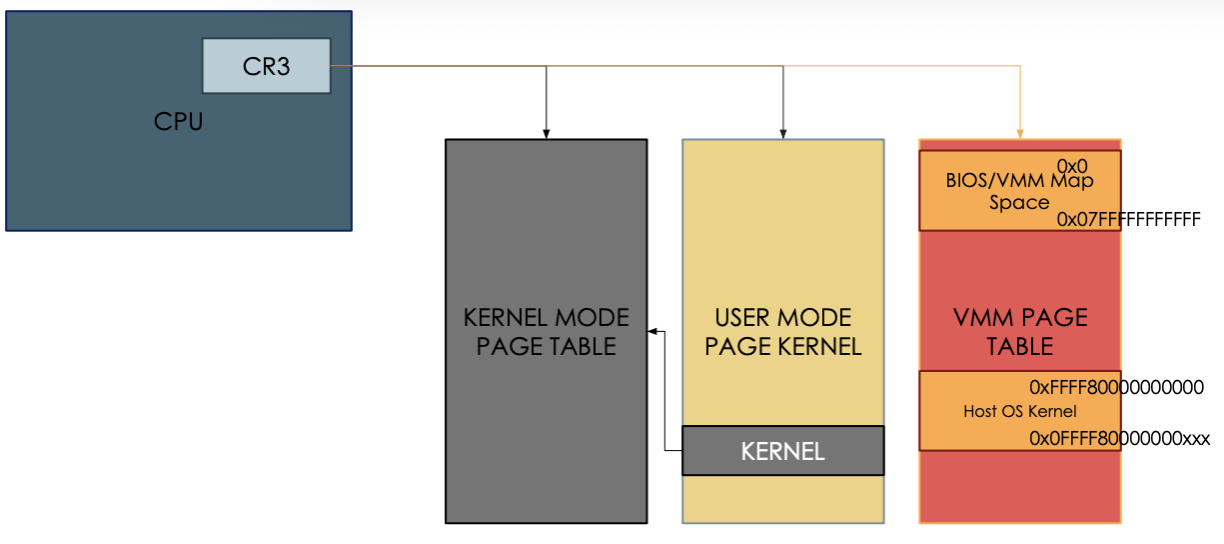
\includegraphics[width=0.45\textwidth]{06-InformeFinal-Latex/img/mapaMemoria.png}
	\caption{Exemple de figura}
	\label{mapesMemoria}
\end{figure}

Tenint en compte la documentació de l’hipervisor i com queda la nova distribució, seria possible accedir als espais de memòria del nucli a travès de l’hipervisor, complint també els permissos necessaris per poder llegir les pàgines protegides del kernel segons els anells de protecció establerts a Linux.
Els anells de protecció serveixen perquè el nucli pugui distingir els privilegis d’on provenen les crides al sistema, d’aquesta manera si s’intenta accedir des d’un posició no privilegiada a un recurs privilegiat, es produirà un error. A la gran majoria de nuclis i sobretot a Linux es sol utilitzar sovint ring 0 i ring 3 on es diferencia de l’espai del nucli i l’espai d’usuari, permetent desde la capa interior accedir a les exterior però no a l’inrevès. S’estableix així una capa de seguretat on també accesos amb privilegis ring 1 i 2 poden interaccionar directament amb el hardware però nomès l’anell interior pot modificar les funcions software més crítiques.
Quan es fa ús del bare-metal hipervisor el que busquem és crear una nova capa dins de l’anell, elevant totes les altres capes, d’aquesta manera l’hipervisor es situaria a la capa de l’anell ring -1 i tindria accès a totes les capes superiors. A més, el Sistema Operatiu natiu pensarà que té tot el control i es comunica directament amb el hardware.

\begin{figure}[!h]
\centering
	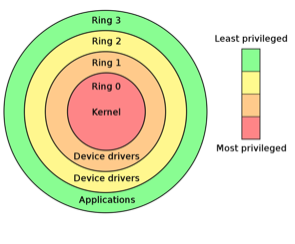
\includegraphics[width=0.45\textwidth]{06-InformeFinal-Latex/img/anellsProteccio.png}
	\caption{Exemple de figura}
	\label{anellsProteccio}
\end{figure}

\subsection{Desament}
L’objectiu aqui és aconseguir guardar els reusltats obtinguts a la tasca superior per tal de poder-los utilitzar i comparar. Hem de pensar que qualsevol emmagatzematge de resultats conté dades sensibles o privilegiades i no han de ser accessibles per l’usuari o des de l’espai de memòria de l’usuari. A mès, també s’ha de decidir en quin format es guarden aquestes dades.

Per saber que hem de guardar, buscarem sempre emmagatzemar el mínim d’informació que ens permeti identificar una modificació en una entrada de taula de pàgina del kernel, per tant, el mínim d’infornació podria estar compost per:
\begin{enumerate}
\item Número de pàgines executables.
\item Direcció física i permissos corresponents.
\item Utilitzar un l’estructura de dades en arbre Merkle Tree, per emmagatzemar el resum hash de la direcció física i permissos o bé el hash del contingut de la direcció física.
\end{enumerate}

Com es pot veure amb la primera opció, no és suficient per identificar una modificació en una entrada de pàgina executable guardar el número d’aquestes, per tant, opció descartada d’inici. La idea que més em convencia era poder montar una estructura de dades en forma d’arbre com el Merkle Tree, de fet, pretenia accedir al contingut de memòria física i fer el resum amb un SHA-256, conjuntament o no amb els permissos de l’entrada de pàgina. Tot i així, recordant que un dels requeriments és que aquest codi pugui còrrer a una impresora, la opció de fer operacions criptogràfiques queda fora de l’abast i per “forta” recomanació , finalment es tria la segona opció on nomès es guardara la direcció física corresponent a l’entrada de la taula de pàgina del kernel i els permissos que conté. Addicionalment, es va cercar un xip que es podria afegir a una impressora a un cost molt baix i que deixaria dur a terme la implementació esmentada [3].
Un cop esmentat el què es guardarà, els tres plantejaments incials per on es guardaran les dades són:



\begin{enumerate}
\item Guardar-ho en un espai de memòria del monitor de la màquina virtual (VMM), semblava
una opció interessant però que no se sap si es pot i s’havia d’investigar.
\item Guardar-ho a l’espai de memòria de l’usuari però protegit amb permissos de superusuari, a priori una opció fàcil i que podria servir per fer proves però poc segura.
\item Guardar-ho al mateix espai de memòria del programa.
\end{enumerate}

El segon dels plantejatments esmentats va ser el primer que se’m va acudir i realment vaig anar directe a provar-ho, la idea principal era volcar tot el que em treia el codi de l’hipervisor en un arxiu, aquesta primera implementació em podria permetre desprès també protegir-lo per superusuari o alguna cosa semblant. Va sorgir d’utiltizar la comanda Linux > a terminal per volcar el que teniem a la terminal a un arxiu quan feia proves. Amb aquesta lògica pretenia crear un fitxer mentres s’executava el codi de detecció i escriure-hi el que anès trobant, però no vaig tenir en compte que des d’on esta situat l’hipervisor, no es disposa d’un sistema de fitxers ja que això està establert pel sistema operatiu i nomès s’entenen els directoris en ell. Ho vaig poder comprovar quan en l’execució del codi l’hipervisor no reconeixia les comandes i les saltava.
En segon lloc, vaig decidir la opció que desprès d’analitzar les tres, sembla més viable per ser una primera implementació. Entenent com a resultats de l’anàlisi les direccions físiques i permissos, guardar totes les dades dels resultats a l’espai de memòria del programa vol dir crear una variable general al nostre programa que sigui accesible per cada una de les iteracions perquè es puguin fer les comprovacions necessàries.
La idea és afegir una variable que emmagatzemi les entrades de totes les taules de pàgina del kernel, una primera implementació més fàcil pot incloure nomès les direccions físiques on estan adreçades i quan es fagin noves iteracions, comprovar si existeix dins d’aquesta variable i la versió final hauria d’incloure una variable de tipus map on les claus serien les direccions físiques i el valor el recull de permissos obtinguts en la detecció.
\section{Comparació de resultats}
\subsection{Accès a les dades existents}
\subsection{Deteccions de modificacions}

\section{Execució en temps real}
Per intentar analitzar el rendiment del codi obtingut s'utilitzen tècniques com l'anàlisi de percentatges d'ús de la CPU o qualsevol tipus de mètrica del processador, això es pot fer a travès de comandes com ara perf stat [], aquestes són eines definides dins del nucli de Linux i analitza els performance counters de la CPU, per tant, s'intenta fer ús d'aquestes mètriques.

La idea principal era observar la càrrega de la CPU perquè quan arribès a un cert valor (threshold) poguessim postposar l’accès a noves direccions físiques, guardant l’estat de per quina direcció anàvem i, quan es poguès reanudar perquè la càrrega de la CPU fòs baixa, es seguiria des del punt on estàvem.
\subsection{Comprovació de rendiment}
Si pensem en com es pot fer ús d'aquestes llibreries podem imaginar-nos que aquestes fan ús de "llibreries" (mirar be aquesta part per defensar com va le proc/stat) que estan situades al kernel de linux i per tant no són accesibles desde el nostre hipervisor que es troba just per sota del SO.

Entre la cerca d'alternatives es mira si l'hipervisor incorpora cap possibilitat d'anàlisi de rendiment de la CPU i nomès es troba una funció que fa un volcatge de tots els registres del processador, es va parlar amb en Rian Quinn (creador de l'hipervisor) i se li pregunta si existeix cap tipus de funcionalitat semblant a la (de KVM mirar esto bn en el foro) i comenta que actualment no existeix cap tipus de funció disponible semblant a nivell d'hipervisor. Una altra opció es basa en seguir un exemple contemplat a l'hipervisor d'interrupció de funcions per part de l'hipervisor, així doncs, es podrien obtenir en temps d'execució els resultats obtenint les adreces de les funcions a l'hora de l'interrupció. Finalment 

 (parlar tambe de poder implementar un sistema amb performance counter com fan els de black hat)
\subsection{Control del codi de detecció}



\section{Conclusions}




\section*{Agraïments}

... ..  .... .. .... ... ..... ... ..... ... ... ..... .... .
.... ..  .... .. .... ... ..... ... ..... ... ... ..... .... .
.... ..  .... .. .... ... ..... ... ..... ... ... ..... .... .
.... ..  .... .. .... ... ..... ... ..... ... ... ..... .... .
.... ..  .... .. .... ... ..... ... ..... ... ... ..... .... .

\begin{thebibliography}{11}
\bibitem{1} Andrew S. Tanenbaum, Maarten Van Steen “Distributed Systems: Principles and Paradigms”, 2nd Ed. Addision-Wesley, Pearson 2007. 
\bibitem{2} https://blog.3mdeb.com/2019/2019-04-30-5-terms-every-hypervisor-developer-should-know/
\bibitem{3} elithecomputerguy. “Episode 328: Introduction to Type 1 Hypervisor Virtualization - Bare Metal Virtual Servers.” YouTube, YouTube, 6 Nov. 2012, www.youtube.com/watch?v=sVTw7sHpnRc.
\bibitem{4} Micha Moffie, Somerville, S. Patent VMM-Based Intrusion Detection System . US 8719936 B2, United States Patent and Trademark Office, 6 May 2014.
\bibitem{5} Black Hat. “Numchecker: A System Approach for Kernel Rootkit Detection.” YouTube, uploaded by Black Hat, 16 Aug. 2016, www.youtube.com/watch?v=TgMsMwsfoQ0.
\bibitem{6} Rian Quinn, 2016 Bareflank (http://bareflank.github.io/hypervisor/)
\bibitem{7} CppCon. “CppCon 2016: Rian Quinn ‘Making C++ and the STL Work in the Linux / Windows Kernels.’” YouTube, YouTube, 6 Oct. 2016, www.youtube.com/watch?v=uQSQy-7lveQ.
\bibitem{8} “Compile/Run Bareflank on Ubuntu 18.04.” YouTube, YouTube, 4 Dec. 2018, www.youtube.com/watch?v=fNLXxtdkhLg.
\bibitem{9} Intel. 2020. Does My Processor Support Intel® Virtualization Technology?. [online] Available at: <https://www.intel.com/content/www/us/en/support/articles/000005486/processors.html> [Accessed 10 November 2020].
\bibitem{10} 3, I., 2020. Intel® 64 And IA-32 Architectures Software Developer Manual: Vol 3. [online] Intel. Available at: <https://www.intel.com/content/www/us/en/architecture-and-technology/64-ia-32-architectures-software-developer-system-programming-manual-325384.html> [Accessed 10 November 2020].
\bibitem{11} Jann Horn, “Meltdown: Reading Kernel Memory from User Space“ , 27th Security Symposium Security 18, 2018 [Abstract] Available: https://meltdownattack.com/meltdown.pdf .[Accessed 18 Nov 2020]
\bibitem{latex} Gitter.im. 2020. Bareflank-Hypervisor/Lobby. [online] Available at: <https://gitter.im/ Bareflank-hypervisor/Lobby> [Accessed 20 December 2020].
\bibitem{12} Bareflank.herokuapp.com. 2020. Join Bareflank On Slack!. [online] Available at: <https:// bareflank.herokuapp.com/> [Accessed 20 December 2020].
\bibitem{13} Microchip.com. 2020. ATECC508A - Crypto Authentication. [online] Available at: <https://www.microchip.com/wwwproducts/en/atecc508a#additional-features> [Accessed 20 December 2020].
\bibitem{14} Linux Documentation, 2020. [online] Available at: <https://www.man7.org/linux/man- pages/man1/perf-stat.1.html> [Accessed 20 December 2020].
\bibitem{15} GitHub. 2020. Hook Exmaple Bareflank. [online] Available at: <https://github.com/ Bareflank/hypervisor/tree/master/examples/hook> [Accessed 21 December 2020].
\bibitem{16} Intel. 2020. [online] Available at: <https://software.intel.com/content/www/us/en/ develop/articles/best-practices-for-paravirtualization-enhancements-from-intel-virtualization- technology-ept-and-vt-d.htm> [Accessed 20 December 2020].l

=


\end{thebibliography}

\appendix

\section*{Apèndix}

\setcounter{section}{1}

\subsection{Secció d'Apèndix}


... ..  .... .. .... ... ..... ... ..... ... ... ..... .... .
.... ..  .... .. .... ... ..... ... ..... ... ... ..... .... .
.... ..  .... .. .... ... ..... ... ..... ... ... ..... .... .
.... ..  .... .. .... ... ..... ... ..... ... ... ..... .... .
.... ..  .... .. .... ... ..... ... ..... ... ... ..... .... .

\subsection{Secció d'Apèndix}


... ..  .... .. .... ... ..... ... ..... ... ... ..... .... .
.... ..  .... .. .... ... ..... ... ..... ... ... ..... .... .
.... ..  .... .. .... ... ..... ... ..... ... ... ..... .... .
.... ..  .... .. .... ... ..... ... ..... ... ... ..... .... .
.... ..  .... .. .... ... ..... ... ..... ... ... ..... .... .


\end{document}

